\newpage
\mysection{Linked Lists}

\begin{figure}[h]
 \centering
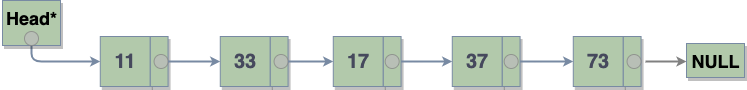
\includegraphics[scale=.40]{images/singly_linked_list.png}
\end{figure}

\mysubsection{Linked Lists in General}

A linked list as a linear collection of data elements whose order is not a contiguous set of memory locations like an array, and who's order is not determined by their actual (physical) location in memory. The order is determined by one element containing the address to the next element in the list. This means nodes in a linked list could be stored in an order that is nothing like we visualize a list as being. The above image is the typical representation of a linked list that abstracts out all of the "address" information. The following image is a similar representation, but showing actual addresses for each node (as well as the address for head).\\

At a minimum, each node contains some data element and a reference (pointer) to the next element in the list. A list can be ordered or unordered depending on needs of implementation. But, one inherent attribute of a linked list is the efficient insertion and deletion of nodes at any an all positions. The structure grows and shrinks with each addition or deletion. One drawback that lists have is the need to access them linearly. When compared to arrays, accessing elements directly (aka random access) is not possible. Another advantage of arrays is they have better cache locality\supcite{Locality63}. \\

A linked list whose nodes contain two fields: an integer value and a link to the next node. The last node is linked to a terminator used to signify the end of the list. Linked lists are among the simplest and most common data structures. They can be used to implement several other common abstract data types, including lists, stacks, queues, associative arrays, and S-expressions, though it is not uncommon to implement those data structures directly without using a linked list as the basis.\\

The principal benefit of a linked list over a conventional array is that the list elements can be easily inserted or removed without reallocation or reorganization of the entire structure because the data items need not be stored contiguously in memory or on disk, while restructuring an array at run-time is a much more expensive operation. Linked lists allow insertion and removal of nodes at any point in the list, and allow doing so with a constant number of operations by keeping the link previous to the link being added or removed in memory during list traversal.\\

On the other hand, since simple linked lists by themselves do not allow random access to the data or any form of efficient indexing, many basic operations—such as obtaining the last node of the list, finding a node that contains a given datum, or locating the place where a new node should be inserted—may require iterating through most or all of the list elements. The advantages and disadvantages of using linked lists are given below. Linked list are dynamic, so the length of list can increase or decrease as necessary. Each node does not necessarily follow the previous one physically in the memory.\\


\begin{minted}[]{c++}
void PrintList(){
    if(!Head){
        cout<<"Empty"<<endl;
        return;
    }else{
        cout<<"The sizeof `Node` in bytes is: "<<sizeof(Head->Data)<<endl;
        cout<<"Address of `Head` is: "<<&Head<<endl;
        cout<<"`Head` points to ->"<<Head<<endl<<endl;
    
        Node *Temp = Head;
        while(Temp != NULL){
            cout<<"|Address: "<<Temp<<" |Data: "<<Temp->Data<<" |Next: "<<Temp->Next<<" | "<<" -> "<<endl;
            Temp = Temp->Next;
        }
        cout<<"NULL"<<endl<<endl;
    }
}
\end{minted}

\textbf{Output:}

\begin{verbatim}
The sizeof `Node` in bytes is: 4
Address of `Head` is: 0x7ffeeeafd550
`Head` points to ->0x7faaf3c05920

|Address: 0x7faaf3c05920 |Data: 1 |Next: 0x7faaf3c05910 |  -> 
|Address: 0x7faaf3c05910 |Data: 56 |Next: 0x7faaf3c05900 |  -> 
|Address: 0x7faaf3c05900 |Data: 20 |Next: 0x7faaf3c058f0 |  -> 
|Address: 0x7faaf3c058f0 |Data: 39 |Next: 0x7faaf3c058e0 |  -> 
|Address: 0x7faaf3c058e0 |Data: 20 |Next: 0x7faaf3c058d0 |  -> 
|Address: 0x7faaf3c058d0 |Data: 56 |Next: 0x0 |  -> NULL
\end{verbatim}

\begin{minted}[]{c++}
struct Node {
    Person Data;
    Node *Next;
    Node(Person p) {
        Data = p;
        Next = NULL;
    }
};

struct Person {
    string Name;
    int Age;
    Person() {
        Name = "";
        Age = 0;
    }
    Person(string n, int a) {
        Name = n;
        Age = a;
    }
};

void Print() {
    Node *Current = Head;
    cout << sizeof(Current->Data) << endl;
    while (Current) {
        cout << "|" << Current->Data.Name << "|" << Current << " ->\n";
        cout ;
        Current = Current->Next;
    }
    cout << "NULL" << endl;
}
\end{minted}

\textbf{Output:}

\begin{verbatim}
40
|Abby|0x8d2200| -> 
|Chuck|0x8d2240| -> 
|Daphne|0x8d23c0| -> 
|Donnie|0x8d2280| -> 
|Echo|0x8d22c0| -> 
|Gerald|0x8d2380| -> 
|MarkyMark|0x8d2300| -> NULL
\end{verbatim}

\mysubsection{Singly Linked Lists}

\begin{center}
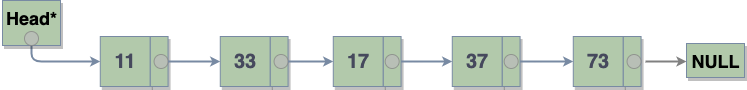
\includegraphics[scale=.40]{images/singly_linked_list.png}
\end{center}

\mysubsection{Circular Linked Lists}
\begin{center}
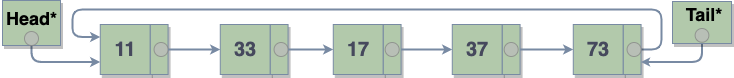
\includegraphics[scale=.40]{images/singly_linked_list_circular.png}
\end{center}


\mysubsection{Doubly Linked Lists}

\begin{center}
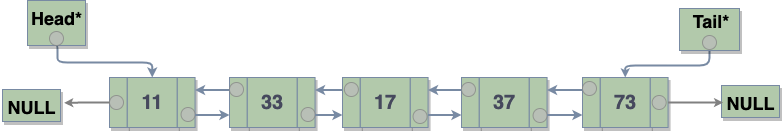
\includegraphics[scale=.40]{images/doubly_linked_list.png}
\end{center}


\mysubsection{Circular Doubly Linked Lists}

\begin{center}
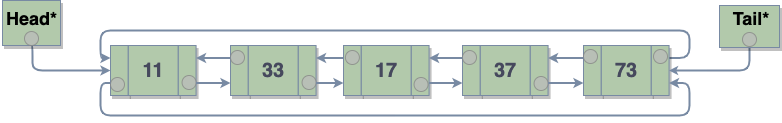
\includegraphics[scale=.40]{images/linked_list_double_circular.png}
\end{center}

